\documentclass{Humantech_Paper_Awardfullpaper_hutech}
\usepackage{bm}
\usepackage{cuted}
\usepackage{graphicx}
\usepackage{caption, subcaption}
\usepackage{setspace}

\title{베지어 곡면을 이용한 3D 모델링}

\begin{document}
\setstretch{1.2}
\fontdimen2\font=1ex
\thispagestyle{firstpage}
	
\begin{strip}
	\maketitle
	\begin{abstract} \raggedright
		공학 설계를 하는 CAGD 분야에서 자동차 차체, 비행기 기체 등을 설계할 때 베지어 곡면을 많이 사용한다. 그 이유는 베지어 곡면은 삼각형 분할에 비해 부드러운 곡면을 표현함에 더 강하고, 적은 메모리를 필요로 한다는 장점이 있기 때문이다. 본 연구에서는 obj파일로 주어진 3D 모델을 베지어 곡면을 이용해 근사하고 압축해 메모리를 줄이는 새로운 방법을 다룬다. 실제로 구면에 이 방법을 적용했을 때, 적당한 오차에 대해 1분 안에 메모리가 200배 이상 감소했다. 본 연구는 3차원 공간상의 볼록 집합의 경계를 대상으로 하며 기존의 베지어 곡면을 이용한 point cloud(물체의 경계를 나타내는 점들)의 근사 방법을 확장해 연구했다. 3차 이상의 고차 베지어 곡면은 활용성이 높지만 계산량이 많다는 단점이 있기 때문에 $\bm{(2, 2)}$차 베지어 곡면을 이용하였으며, 낮은 차수로도 좋은 결과를 얻었다. 우리는 곡면을 근사하기 위해 point cloud를 원통형으로 분할하는 과정을 거쳤다. 분할한 각 영역의 점들을 하나의 베지어 곡면으로 근사하였고, 공간상에서 광선(직선)과 삼각형의 교점을 찾는 Möller–Trumbore intersection algorithm과 선행 연구를 참고해 최소제곱법, 가우스-뉴턴 방법을 사용하여 효율적으로 근사가 되도록 하였다. 베지어 곡면과 원 곡면의 차이를 나타내는 오차함수는 하우스도르프 거리가 적합하지만, 계산량이 너무 많다는 단점이 있다. 때문에 이를 적절히 변형해 새로운 오차함수를 만듦으로써 적은 시간을 소모하게 만들었다. 더 나아가 연구 대상으로 하는 모든 곡면을 충분히 근사할 수 있음을 수학적으로 증명하였다. 이러한 수학적 근거와 프로그래밍 효율성에 기반한 본 연구의 곡면 모델링은 VR, AR 및 홀로그램 분야에 크게 기여할 것으로 기대된다. 또한 CAGD 분야에서 더 큰 활용이 가능하며 미래 우주 공학과도 직결되는 우주선이나 우주 정거장을 디자인하는 데도 사용될 수 있다.
	\end{abstract}
\end{strip}
	
\section{서론}
3D 프린터, 홀로그램 및 VR과 AR은 지금도 활발하게 사용되고 있는 기술이고 미래 전망도 좋다. 이들이 실제로 상용화되기 위해선 보다 효율적으로 곡면을 다루기 위한 컴퓨터 그래픽 기술이 필수적이다. 

현재 3D 모델을 저장하기 위해 obj파일이 흔히 사용된다. obj파일은 곡면을 표현하기 위해 삼각형 혹은 사각형 분할을 이용한다. 이러한 다각형 분할은 베지어 곡면을 이용한 압축에 비해 구면과 같은 부드러운 곡면을 표현하는 능력이 떨어진다. 또한 베지어 분할은 베지어 곡면이 가지는 조절점이라는 고유한 성질 덕에 메모리도 적게 소모한다. 

본 연구는 obj파일 형식으로 주어진 3차원 공간상의 곡면을 조각별로 분할하여 베지어 곡면을 통해 근사 및 압축하는 방법을 제시한다. 이는 obj파일에 비해 메모리 측면에서의 이점을 가진다. 혹은 자동차, 선박, 비행기 등을 설계할 때 이용되는 CAD(Computer Aided Design) 중에서도 수학적인 도구를 이용하는 CAGD 분야에서의 활용이 기대된다. 
	
\section{이론적 배경}
\subsection{베지어 곡선과 베지어 곡면}
\begin{defn}
	\textbf{$\bm{n}$차 베지어 다항식(Bézier polynomial)}은 $(n+1)$개의 점 $\mathbf{P}_0, \mathbf{P}_1, \cdots, \mathbf{P}_n$에 대해 다음과 같이 주어진다.
	\begin{equation} \label{BezierCurve}
		\mathbf{B}(t)=\sum_{i=0}^n \binom ni(1-t)^{n-i}t^i\mathbf{P}_i
	\end{equation}
	
	\noindent 이때 $n$차 베지어 다항식에 의한 구간 $[0, 1]$의 상을 \textbf{$\boldsymbol{n}$차 베지어 곡선(Bézier curve)}이라 한다. 또한 점 $\mathbf{P}_0, \cdots, \mathbf{P}_n$을 이 베지어 곡선의 \textbf{조절점(control point)}이라 한다. 
\end{defn}

\begin{defn}
	$(n+1)(m+1)$개의 점 $\mathbf{b}_{ij}\ (i = 0, 1, \cdots, n \ \text{and} \ j = 0, 1, \cdots, m)$에 대해 다음 $2$변수 다항식을 생각하자. 
	\begin{equation} \label{BezierSurface}
		\mathbf{x}(u, v)=\sum_{i=0}^n\sum_{j=0}^m B_i^n(u)B_j^m(v)\mathbf{b}_{ij} 
	\end{equation}

	여기서 Bernstein 다항식 $B_i^n(t)=\binom ni(1-t)^{n-i}t^i$로 주어진다. $\mathbf{x}$에 의한 단위 정사각형 $[0, 1]^2$의 상을 \textbf{$\bm{(n, m)}$차 베지어 곡면(Bézier surface)}이라 한다. 마찬가지로 점 $\mathbf{b}_{ij}$를 이 베지어 곡면의 \textbf{조절점}이라 한다 \cite{Farin}.
\end{defn}

\begin{figure}[h]
	\begin{center}
{\tiny }		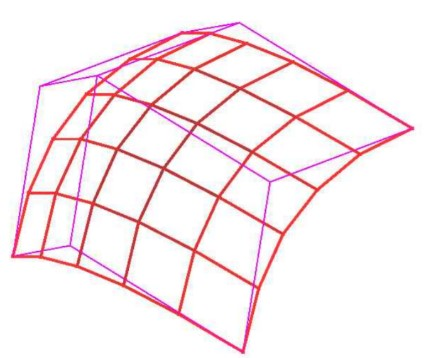
\includegraphics[width=.25\textwidth]{BezierSurface}
	\end{center} \setstretch{1.2}
	\raggedright \small \textbf{Fig. 1. $\bm{(2, 2)}$차 베지어 곡면.} $(2, 2)$차 베지어 곡면(빨간색)과 조절점 $\mathbf{b}_{ij}$를 연결한 선분(보라색).
\end{figure}

본 연구에서는 $(2, 2)$차 베지어 곡면을 이용한다. 

\subsection{경계}
\begin{defn}
	위상공간 $(X, \mathfrak{I})$의 부분집합 $A$의 \textbf{내부(interior)}와 \textbf{폐포(closure)}, \textbf{경계(boundary)}는 각각 다음과 같이 정의된다 \cite{Munkres}.
	\begin{align*}
		A^\circ &= \bigcup \{ U \subset A \mid U \in \mathfrak{I} \} \\
		\bar{A} &= \bigcap \{ C \subset A \mid X-C \in \mathfrak{I} \} \\
		\partial A &= \bar{A} - A^\circ
	\end{align*}
\end{defn}

특히 $\bar{A}$는 $A$의 원소 $A$의 극한점(limit point)들로 이루어진다. 

\subsection{볼록집합}
\begin{defn}
	$\mathbb{R}^n$의 부분집합 $C$가 다음 조건을 만족할 때, $C$를 \textbf{볼록집합(convex set)}이라 부른다. 
	\begin{equation*}
		\forall \mathbf{x}, \mathbf{y} \in C,\ \forall t \in [0, 1],\ (1-t)\mathbf{x}+t\mathbf{y} \in C
	\end{equation*}
\end{defn}

\begin{lem} \label{closureofconvexset}
	$C \subset \mathbb{R}^n$가 볼록집합이면, $C$의 폐포(closure) $\bar{C}$도 볼록집합이다. 
\end{lem}
\begin{proof}
	임의의 $\mathbf{x}, \mathbf{y} \in \bar{C}$와 $t \in [0, 1]$에 대해 $(1-t)\mathbf{x} + t\mathbf{y} \in \bar{C}$임을 보이자. $\mathbf{x}, \mathbf{y} \in \bar{C}$이므로 적당한 수열 $\{ \mathbf{x}_n \}, \{ \mathbf{y}_n \} \subset C$이 존재해 $\mathbf{x}_n \to \mathbf{x}, \, \mathbf{y}_n \to \mathbf{y}$를 만족한다. 각 자연수 $n$에 대해 $\mathbf{x}_n$과 $\mathbf{y}_n$은 볼록집합 $C$의 원소이므로 $(1-t)\mathbf{x}_n + t\mathbf{y}_n \in C$이다. 이제 $n \to \infty$의 극한을 취하면 $(1-t)\mathbf{x} + t\mathbf{y} \in \bar{C}$를 얻는다. 
\end{proof}

\begin{thm} \label{homeo}
	$\mathbb{R}^n$의 볼록집합 $C$가 유계이고 $\mathbf{0} \in C^\circ$를 만족한다고 하자. 함수 $\phi \colon \partial C \to S^{n-1}$를 $\phi(\mathbf{x}) = \mathbf{x} / \Vert \mathbf{x} \Vert$로 정의하면 $\phi$는 위상동형사상이다. 이때 $S^{n-1} = \{ \mathbf{x} \in \mathbb{R}^n \mid \Vert \mathbf{x} \Vert = 1 \}$은 $(n-1)$차원 단위 구면이다 \cite{convex}.
\end{thm}

\subsection{뉴턴-랩슨 방법과 가우스-뉴턴 방법}
\textbf{뉴턴-랩슨 방법}은 미분가능한 실수값 함수의 근 $\hat{x}$을 찾는 알고리즘이다. 함수 $f\colon(a, b)\to\mathbb{R}$과 도함수 $f^\prime$에 대해, 현재 $f(x)=0$의 해의 근사치를 $x_n$이라 하자. $f$의 선형 근사는 다음과 같다.
\begin{equation*}
	y=f^\prime(x_n)(x-x_n)+f(x_n)
\end{equation*}

다음 근사치 $x_{n+1}$은 위 직선의 $x$절편으로 주어진다.
\begin{equation} \label{newton}
	x_{n+1}=x_n-\frac{f(x_{n})}{f^\prime(x_n)}
\end{equation}

초기값 $x_0$부터 시작해 \eqref{newton}을 반복해 더 좋은 근사치를 얻을 수 있다. $f$가 두 번 연속적으로 미분가능하면 뉴턴-랩슨 방법은 이차 근사임이 알려져 있다. 즉 $\vert x_{n+1} - \hat{x} \vert \leq C \vert x_n - \hat{x} \vert ^2$를 만족하는 양수 $C$가 존재한다. \\

\textbf{가우스-뉴턴 방법}은 뉴턴-랩슨 방법을 다변수 벡터함수로 확장한 것이다. 함수 $\mathbf{f} \colon \mathbb{R}^n \to \mathbb{R}^m$에 대해 $\mathbf{f}(\mathbf{x}) = \mathbf{0}$의 해의 근사치를 $\mathbf{x}_n$이라 하자. 뉴턴-랩슨 방법과 비슷하게 $\mathbf{x}_n$에서 $\mathbf{f}$의 선형 근사를 구한다. 
$$ \mathbf{f}(\mathbf{x}) \approx \mathbf{f}(\mathbf{x}_n) + \mathbf{J}_{\mathbf{f}}(\mathbf{x}_n) (\mathbf{x} - \mathbf{x}_n) $$
이때 $\mathbf{f}$의 \textbf{야코비 행렬(Jacobian matrix)} $\mathbf{J}_{\mathbf{f}}$는 다음과 같은 $m \times n$ 행렬이다. 
$$ \mathbf{J}_{\mathbf{f}}= \begin{pmatrix} \partial f_1 / \partial x_1 & \partial f_1 / \partial x_2 & \cdots & \partial f_1 / \partial x_n \\ \partial f_2 / \partial x_1 & \partial f_2 / \partial x_2 & \cdots & \partial f_2 / \partial x_n \\ \vdots & \vdots & \ddots & \vdots \\ \partial f_m / \partial x_1 & \partial f_m / \partial x_2 & \cdots & \partial f_m / \partial x_n \end{pmatrix}$$

$\mathbf{f}(\mathbf{x}_{n+1}) = \mathbf{0}$이라 하면 $\mathbf{J}_{\mathbf{f}}(\mathbf{x}_n) (\mathbf{x}_{n+1} - \mathbf{x}_n) = -\mathbf{f}(\mathbf{x}_n)$이고, 양변에 $\mathbf{J}_\mathbf{f}$의 의사역행렬(pesudo-inverse)를 곱해 다음 해의 근사치를 얻는다. 
$$ \mathbf{x}_{n+1} = \mathbf{x}_n - (\mathbf{J}_{\mathbf{f}}(\mathbf{x}_n)^\intercal \mathbf{J}_{\mathbf{f}}(\mathbf{x}_n))^{-1} \mathbf{J}_{\mathbf{f}}(\mathbf{x}_n)^\intercal \mathbf{f}(\mathbf{x}_n) $$

실제로 $m = n = 1$이라면 이는 뉴턴-랩슨 방법과 같다.

\subsection{하우스도르프 거리}
\begin{defn}
	거리공간 $(M, d)$의 공집합이 아닌 두 부분집합 $X, Y$에 대해 하우스도르프 거리는 다음과 같이 주어진다 \cite{Munkres}.
	\begin{equation} \label{hausdorffdistance}
		d_H(X, Y) = \max \left\{ \sup_{x \in X} \inf_{y \in Y} d(x, y), \, \sup_{y \in Y} \inf_{x \in X} d(x, y) \right\}
	\end{equation}
\end{defn}

하우스도르프 거리는 거리공간 상에서 두 집합이 서로 떨어진 정도를 나타낸다. 실제로, $d_H(X, Y) = 0$일 필요충분조건은 $X$와 $Y$의 폐포가 일치하는 것이다. 

\subsection{obj파일}
obj는 3D 이미지를 저장하는 표준적인 파일이다. obj 파일은 정점 $v$, 단위 법선벡터 $v_n$, 텍스쳐 $v_t$, 면 $F$로 이루어진다. 먼저 $v, v_n, v_t$의 $x, y, z$성분이 차례로 주어진다. 마지막에 $F$가 주어지는데, 각각의 $F$는 $v / v_n / v_t$ 블록 3개 또는 4개로 이루어진다. 3개면 삼각형 면, 4개면 사각형 면이다. 

앞으로 obj파일의 정점 $v$를 $\mathbf{P}_k$로 나타낸다. 그리고 obj파일로 주어진 곡면은 면 $F$들의 합집합을 의미한다. 

\section{연구 결과}
\subsection{분할 방법}
정점들을 하나의 베지어 곡면으로 근사한다면 오차가 너무 커진다. 그래서 정점들이 놓여있는 공간을 원통형으로 분할하고, 각 분할된 곡면을 하나의 베지어 곡면으로 근사한다. 원통형 분할은 원통형 좌표계 $(r, \theta, z)$를 기준으로 $\theta$와 $z$의 범위를 이등분하며 이루어진다. 

\begin{figure}[h]
	\begin{center}
		\begin{subfigure}{.15\textwidth}
			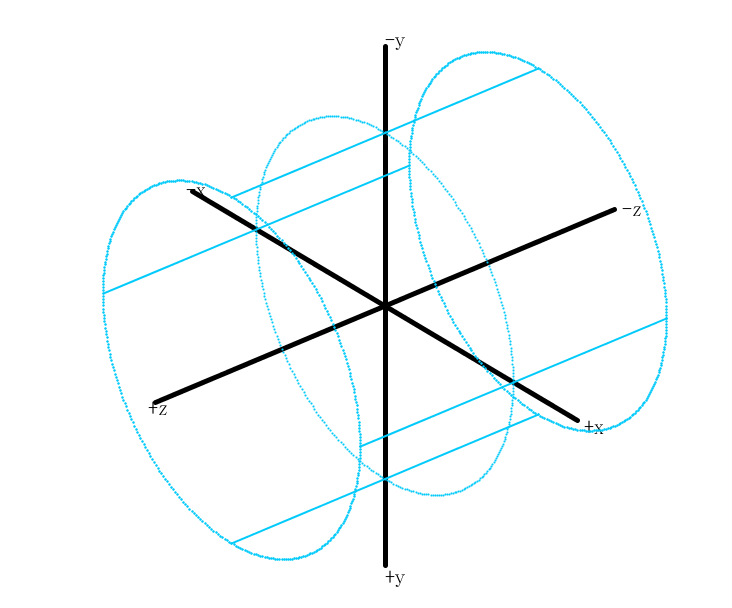
\includegraphics[width=\textwidth]{subdivision1}
			\caption{$n=1$}
		\end{subfigure}
		\begin{subfigure}{.15\textwidth}
			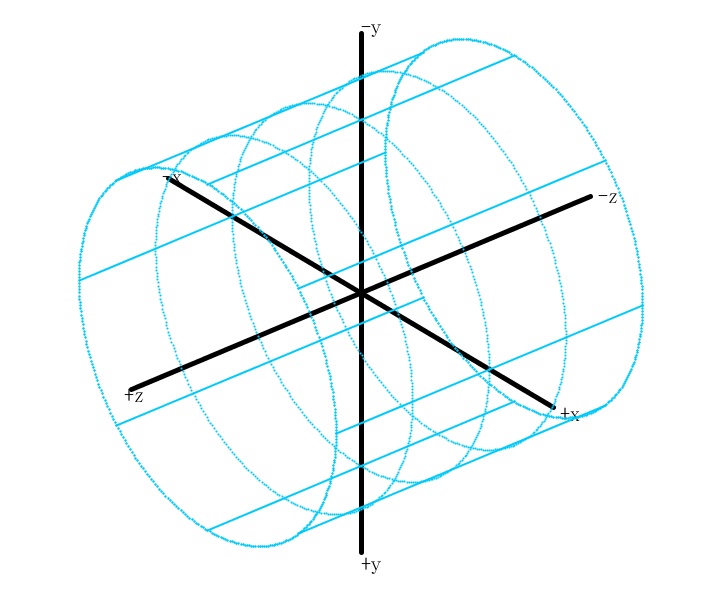
\includegraphics[width=\textwidth]{subdivision2}
			\caption{$n=2$}
		\end{subfigure}
		\begin{subfigure}{.15\textwidth}
			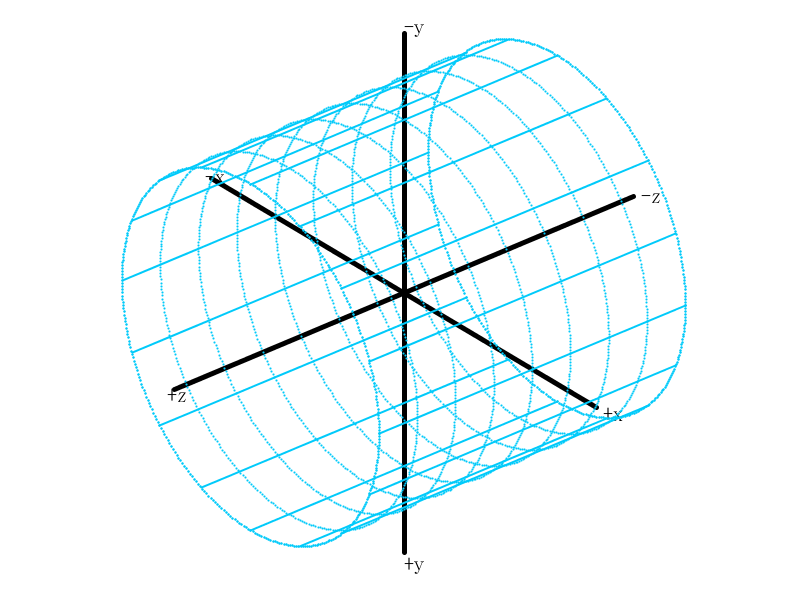
\includegraphics[width=\textwidth]{subdivision3}
			\caption{$n=3$}
		\end{subfigure}
	\end{center} \setstretch{1.2}
	\raggedright \small \textbf{Fig. 2. 원통형 분할.} 원통형 분할은 $\theta$와 $z$의 범위를 이등분하며 이루어진다. 그림에서는 $\theta$와 $z$의 범위를 각각 $2^{n+1}$, $2^n$등분했다. 
\end{figure}

원통형 분할은 같은 $(\theta, z)$를 가지는 두 점이 존재하면 근사가 제대로 이루어지지 않는다는 단점이 있다. 그래서 연구 대상을 내부가 공집합 아닌 $\mathbb{R}^3$의 유계 볼록 집합의 경계로 제한한다. 정리 \ref{homeo}에 의해 이는 2차원 곡면이 된다. 

하지만 기울어진 타원체를 생각하면, 이는 분명 $\mathbb{R}$의 볼록 집합의 경계이지만 같은 $(\theta, z)$를 가지는 두 점이 존재함을 알 수 있다. 이런 문제를 해결하고자, 사전작업으로 거리가 가장 먼 두 점을 $z$축 위에 올린다. 두 점을 각각 $(x_1, y_1, z_1), \, (x_2, y_2, z_2)$라 하자. 우선 평행변환을 이용해 두 점의 중점이 원점이 되도록 한다. 
$$ \mathbf{P}_k \ \leftarrow \ \mathbf{P}_k - \left( \frac{x_1 + x_2}2, \, \frac{y_1 + y_2}2, \, \frac{z_1 + z_2}2 \right)^\intercal $$
	
그리고 $xy$회전, $zx$회전을 통해 두 점이 $z$축 위에 올라가도록 한다. 각각 다음과 같다. (평행변환과 회전변환을 할 때마다 $x_i, y_i, z_i$의 값이 바뀐다. 아래 수식의 $x_i, y_i, z_i$는 시행을 하는 상태에서의 값을 말한다.)

$$ \mathbf{P}_k\ \leftarrow\ \begin{pmatrix}
	x_1 & y_1 & 0 \\ -y_1 & x_1 & 0 \\ 0 & 0 & 1
\end{pmatrix} \mathbf{P}_k $$
$$ \mathbf{P}_k\ \leftarrow\ \begin{pmatrix}
	z_1 & 0 & -x_1 \\ 0 & 1 & 0 \\ x_1 & 0 & z_1
\end{pmatrix} \mathbf{P}_k $$

사전작업을 마친 후 거리가 가장 먼 두 점의 좌표를 $(0, 0, \pm h)$라 하자. 이를 원통형으로 분할하면 각 영역은 $\theta_a \leq \theta \leq \theta_{a+1}, \, z_b \leq z \leq z_{b+1}$로 표현된다. 이때 $0 \leq a, b < 2^n$에 대해 $\theta_a, z_b$는 각각 다음과 같다. 

$$ \theta_a = \frac{2\pi a}{2^n}, \quad z_b = -h + \frac{2hb}{2^n} $$

사전작업을 통해 같은 $(\theta, z)$를 가지는 두 점이 존재하지 않는다는 사실을 알 수 있다. 

\begin{thm} \label{proj}
	볼록집합 $C \subset \mathbb{R}^3$에 대해 obj파일로 주어진 곡면을 경계 $\partial C$라 하자. 다음과 같이 정의된 함수 $\mathbf{f} \colon [0, 2\pi] \times [-h, h] \to \partial C$는 잘 정의되며, 전사(surjective)이다. 
	$$ \mathbf{f}(\theta_0, z_0) = (\partial C \text{위의 점 중 } \theta = \theta_0, \, z = z_0 \text{인 점}) $$
	(이때 $r=0$인 점은 어떤 $\theta = \theta_0$도 만족한다고 생각한다.)
\end{thm}
\begin{proof}
	우선 $\partial C$는 닫힌 곡면이므로 정의역의 모든 점이 공역의 적어도 하나의 점에 대응된다는 것은 자명하다. $\mathbf{f}$가 전사임을 보이기 위해 $\partial C$의 모든 점이 $-h \leq z \leq h$ 범위에 있음을 보이면 충분하다. 어떤 점이 $z > h$ 범위에 있다고 가정하자. $\partial C$는 $\mathbf{P}_k$를 꼭짓점으로 하는 다각형 면들의 합집합이므로, 적어도 하나의 정점 $\mathbf{P}_k$가 $z > h$ 범위에 존재해야 한다. 그런데 이는 거리가 가장 먼 두 점이 $(0, 0, \pm h)$라는 사실에 모순이다. 
	
	$(0, 0, \pm h)^\intercal$은 $\partial C$ 위의 점이므로 $\bar{C}$의 원소이다. 보조정리 \ref{closureofconvexset}에 의해 $\bar{C}$는 볼록집합이고, 따라서 $\mathbf{0} \in \bar{C}$이다. 여기서 우리는 $\mathbf{0} \in C^\circ$라고 가정할 수 있다. 또한 $\{ (0, 0, z)^\intercal \mid -h < z < h \} \subset C^\circ$이다. 
	
	$(\theta, z) = (\theta_0, z_0)$를 만족하는 서로 다른 두 점이 있다고 가정하자. $z_0 = \pm h$이면 이에 대응되는 점은 하나뿐이므로 $-h < z_0 < h$이다. $(0, 0, z_0)$는 $C$의 내부에 있고, 이를 기준으로 정리 \ref{homeo}을 사용하면 $\phi$에 의해 두 점이 같은 점으로 사영되므로 모순이 발생한다. 따라서 $\mathbf{f}$는 잘 정의되며 전사함수이다. 
\end{proof}

또한 $\partial C$는 닫힌 곡면이므로 $\mathbf{f}$는 연속함수이다. $\mathbf{f}$가 연속이 아니라면 $\partial C$가 연속적으로 매개화될 수 없고, 곡면이 아니다. 

\subsection{근사 방법}
분할된 영역의 곡면을 하나의 베지어 곡면으로 근사한다. 각 영역의 베지어 곡면이 연속적으로 이어지기 위해서는 베지어 곡면의 네 모서리($u=0, \, u=1, \, v=0, \, v=1$)가 영역의 경계에 위치해야 한다. 특히 네 조절점 $\mathbf{b}_{00} = \mathbf{x}(0, 0), \, \mathbf{b}_{02} = \mathbf{x}(0, 1), \, \mathbf{b}_{20} = \mathbf{x}(1, 0), \, \mathbf{b}_{22} = \mathbf{x}(1, 1)$는 각각 4개의 영역이 만나는 경계에 위치한다. 

분할된 영역이 $\theta_a \leq \theta \leq \theta_{a+1}, \, z_b \leq z \leq z_{b+1}$로 주어진다고 하자. 반직선 $\ell_{ab} \colon \theta = \theta_a, \, z = z_b$로 정의하고, 네 반직선 $\ell_{ab}, \, \ell_{a, \, b+1}, \, \ell_{a+1, \, b}, \, \ell_{a+1, \, b+1}$과 obj파일의 면 $F$의 교점을 찾아 각각 $\mathbf{b}_{00}, \mathbf{b}_{02}, \mathbf{b}_{20}, \mathbf{b}_{22}$로 둔다. 이때 광선 또는 직선과 삼각형의 교점을 찾는 빠른 알고리즘인 Möller-Trumbore intersection algorithm을 이용한다 \cite{raytriangle}.

Möller-Trumbore intersection algorithm을 이용하면 영역의 경계 $\theta_a \leq \theta \leq \theta_{a+1}, \, z = z_b$와 $F$의 교선을 찾을 수 있다. 식 (eqref{BezierSurface}로 매개화되는 베지어 곡면에서 $u = 0$인 부분은 $\mathbf{b}_{00}, \mathbf{b}_{01}, \mathbf{b}_{02}$를 세 조절점으로 가지는 $2$차 베지어 곡선이다. 따라서 다음 2차 베지어 곡선의 성질을 이용하면 $\mathbf{b}_{01}$을 얻을 수 있다. 

\begin{thm}
	공간상의 세 점 $\mathbf{P}_0, \mathbf{P}_1, \mathbf{P}_2$를 조절점으로 가지는 2차 베지어 곡선을 생각하자. $\mathbf{P}_0$과 $\mathbf{P}_2$를 잇는 직선에서 가장 멀리 떨어진 베지어 곡선 위의 점을 $\mathbf{Q}$라 하면 $\mathbf{Q}$는 $\mathbf{P}_1$과 $(\mathbf{P}_0 + \mathbf{P}_2) / 2$의 중점이다 \cite{last year}.
\end{thm}
\begin{proof}
	우선 2차 베지어 곡선은 다음과 같이 주어진다. 
	\begin{align*}
		\mathbf{B}(t) &= (1-t)^2 \mathbf{P}_0 + 2t(1-t) \mathbf{P}_1 + t^2 \mathbf{P}_2 \\
		&= (1-t)((1-t)\mathbf{P}_0 + t\mathbf{P}_1) + t((1-t)\mathbf{P}_1 + t\mathbf{P}_2)
	\end{align*}
	
	세 점 $\mathbf{P}_0, \mathbf{P}_1, \mathbf{P}_2$는 하나의 평면 $\alpha$를 결정한다. $(1-t)\mathbf{P}_0 + t\mathbf{P}_1$과 $(1-t)\mathbf{P}_1 + t \mathbf{P}_2$는 각각 $\mathbf{P}_0$와 $\mathbf{P}_1$, $\mathbf{P}_1$과 $\mathbf{P}_2$의 $t \colon (1-t)$ 내분점이므로 $\alpha$ 위에 있다. 또한 $\mathbf{B}(t)$도 $\alpha$ 위에 있고, 따라서 2차 베지어 곡선은 하나의 평면에 놓여있다. 
	
	이 평면 위에서 다음을 만족하는 직교좌표계 $(x^\prime, y^\prime)$를 만들 수 있다.
	$$ \mathbf{P}_0 = \begin{pmatrix} -a \\ 0 \end{pmatrix}, \quad \mathbf{P}_1 = \begin{pmatrix} b \\ c \end{pmatrix}, \quad \mathbf{P}_2 = \begin{pmatrix} a \\ 0 \end{pmatrix}, \quad (a, b, c > 0) $$
	그러면 $\mathbf{Q}$는 $y^\prime$좌표가 최대인 점이다. $\mathbf{B}(t)$의 $y^\prime$좌표는 $2ct(1-t)$이므로, $t = 1/2$일 때 최대이다. $\mathbf{Q} = \mathbf{B}(1/2) = (b/2, \, c/2)^\intercal$이므로 위 정리가 성립한다. 
\end{proof}

따라서 영역의 경계 $\theta_a \leq \theta \leq \theta_{a+1}, \, z = z_b$와 $\partial C$의 교선을 잡고, 교선 위의 점들 중 $\mathbf{b}_{00}$과 $\mathbf{b}_{02}$를 잇는 직선에서 가장 멀리 떨어진 점 $\mathbf{Q}$를 찾는다. 그러면 $\mathbf{b}_{01} = 2\mathbf{Q} - (\mathbf{b}_{00} + \mathbf{b}_{02})/2$로 주어진다. 같은 방법으로 조절점 $\mathbf{b}_{01}, \mathbf{b}_{10}, \mathbf{b}_{12}, \mathbf{b}_{21}$을 얻을 수 있다. 

\begin{figure}[h]
	\begin{center}
		\begin{subfigure}{.2\textwidth}
			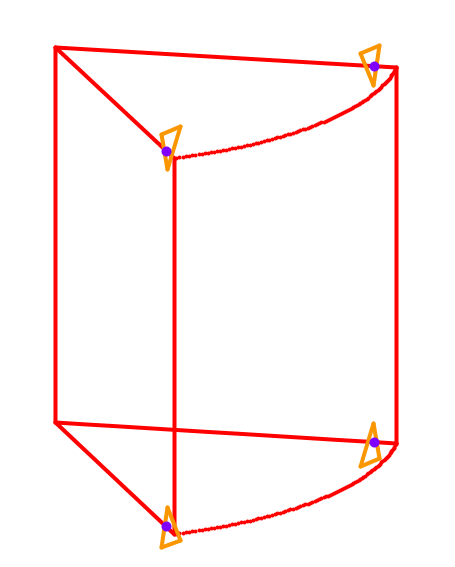
\includegraphics[width=\textwidth]{approx1}
			\caption{$\mathbf{b}_{00}, \mathbf{b}_{02}, \mathbf{b}_{20}, \mathbf{b}_{22}$}
		\end{subfigure}
		\begin{subfigure}{.2\textwidth}
			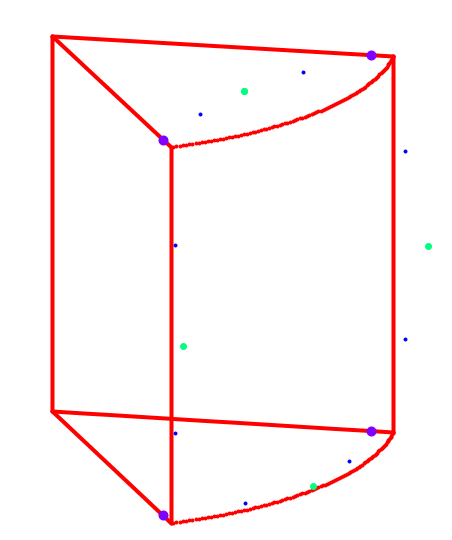
\includegraphics[width=\textwidth]{approx2}
			\caption{$\mathbf{b}_{01}, \mathbf{b}_{10}, \mathbf{b}_{12}, \mathbf{b}_{21}$}
		\end{subfigure}
	\end{center} \setstretch{1.2}
	\raggedright \small \textbf{Fig. 3. 조절점 - $\mathbf{b}_{11}$ 제외.} $\mathbf{b}_{11}$을 제외한 조절점을 얻기 위해 Möller-Trumbore intersecton algorithm을 이용한다. (a) 네 영역이 만나는 (반)직선과 obj파일의 면 $F$의 교점으로 $\mathbf{b}_{00}, \mathbf{b}_{02}, \mathbf{b}_{20}, \mathbf{b}_{22}$를 얻는다. (b) 영역의 경계와 $F$의 교선을 잡고, 2차 베지어 곡선을 성질을 이용해 $\mathbf{b}_{01}, \mathbf{b}_{10}, \mathbf{b}_{12}, \mathbf{b}_{21}$를 구한다. 
\end{figure}

이제 조절점 $\mathbf{b}_{11}$을 구하기 위해 최소제곱법과 가우스-뉴턴 방법을 이용한다. 이 아이디어는 선형 연구를 참고했다 \cite{2021}. 영역 내의 정점을 $\mathbf{P}_k \ (k=1, 2, \cdots, K)$라 하자. 각 $\mathbf{P}_k$에 대응되는 베지어 곡면의 매개변수 $u_k$와 $v_k$가 주어졌다고 가정한다. $\mathbf{x}_k = \mathbf{x}(u_k, v_k)$에서 이미 알고 있는 조절점들에 대한 항을 $\mathbf{y}_k$로 두면 다음과 같이 나타날 수 있다.

$$ \mathbf{x}_k = \mathbf{x}(u_k, v_k) = B_1^2(u_k) B_1^2(v_k) \mathbf{b}_{11} + \mathbf{y}_k $$ 

$\mathbf{b}_{11}$에 관한 연립방정식 $\mathbf{x}_k = \mathbf{P}_k \ (1 \leq k \leq K)$는 일반적으로 해를 가지지 않는다. 따라서 제곱오차 $S = \sum_{k=1}^K \Vert \mathbf{x}_k - \mathbf{P}_k \Vert^2$을 최소로 만드는 $\mathbf{b}_{11}$의 값을 구한다. 이를 위해 $x, y, z$ 좌표로 나눠 행렬방정식으로 표현한다. 

\begin{align*}
	&\begin{pmatrix}
		B_1^2(u_1)B_1^2(v_1) \\ B_1^2(u_2)B_1^2(v_2) \\ \vdots \\ B_1^2(u_K)B_1^2(v_K)
	\end{pmatrix} \begin{pmatrix}
		b_{11}^x & b_{11}^y & b_{11}^z
	\end{pmatrix} \\
	&= \begin{pmatrix}
		P_1^x-y_1^x & P_1^y-y_1^y & P_1^z-y_1^z \\ P_2^x-y_2^x & P_2^y-y_2^y & P_2^z-y_2^z \\ \vdots & \vdots & \vdots \\ P_K^x-y_K^x & P_K^y-y_K^y & P_K^z-y_K^z
	\end{pmatrix}
\end{align*}

이때 윗첨자 $x, y, z$는 각각 벡터의 $x, y, z$성분을 나타낸다. 위 행렬방정식의 제곱오차도 마찬가지로 $S$임을 알 수 있다. $AX = B$ 꼴의 행렬방정식에서 최소제곱오차를 가지는 $X = (A^\intercal A)^{-1} A^\intercal B$로 주어지므로, 다음과 같이 $\mathbf{b}_{11}$을 구할 수 있다. 
\begin{equation} \label{findb11}
	\mathbf{b}_{11} = \frac{\sum_{k=1}^K B_1^2(u_k) B_1^2 (v_k) (\mathbf{P}_k - \mathbf{y}_k)}{\sum_{k=1}^K (B_1^2(u_k) B_1^2(v_k))^2}
\end{equation}

각 $\mathbf{P}_k$에 대해 대응되는 $u_k$와 $v_k$를 알고 있다면 \eqref{findb11}과 같이 $\mathbf{b}_{11}$을 구할 수 있다. 이제 최적의 $u_k$와 $v_k$를 얻기 위해 가우스-뉴턴 방법을 사용한다. 즉, 각각의 $k$에 대해 $\mathbf{x}_k$와 $\mathbf{P}_k$의 차이를 줄이는 방향으로 $u_k$와 $v_k$를 갱신한다. 현재 $u_{n, \, k}$와 $v_{n, \, k}$의 값이 $\mathbf{u}_{n, \, k} = (u_{n, \, k}, v_{n, \, k})^\intercal$로 주어질 때, 다음과 같이 $\mathbf{u}_{n+1, \, k}$를 알 수 있다. 

\begin{equation} \label{rearrange}
	\mathbf{u}_{n+1, \, k} = \mathbf{u}_{n, \, k} - (\mathbf{J}_\mathbf{x}^\intercal \mathbf{J}_\mathbf{x})^{-1} \mathbf{J}_\mathbf{x}^\intercal (\mathbf{x}_k - \mathbf{P}_k)
\end{equation}

이때 $\mathbf{J}_\mathbf{x}$는 $\mathbf{u} = (u, v)^\intercal$에 대한 $\mathbf{x}$의 Jacobian matrix이다.

$$ \mathbf{J}_\mathbf{x} = \begin{pmatrix} \partial x^x / \partial u & \partial x^x / \partial v \\ \partial x^y / \partial u & \partial x^y / \partial v \\ \partial x^z / \partial u & \partial x^z / \partial v \end{pmatrix} $$ 

앞에서와 마찬가지로 윗첨자는 벡터의 성분을 나타낸다.

초기조건 $u_{0, \, k} = v_{0, \, k} = 0.5$에 대해, 다음 과정을 반복한다. 
\begin{enumerate}
	\item 식 \eqref{findb11}와 같이 $\mathbf{b}_{11}$을 구한다. 
	\item 식 \eqref{rearrange}와 같이 $u_k, v_k$를 갱신한다. 
\end{enumerate}
실험적으로 약 20번 반복하면 충분했다. 그 이상은 위 과정을 반복해도 $u_k$와 $v_k$의 값의 변화가 거의 없었다. 

이때, 베지어 곡면은 $0 \leq u, v \leq 1$의 범위에서 정의되므로 중간 과정에서 $u_{n, \, k}$ 또는 $v_{n, \, k}$가 0.01보다 작아지면 0.01로 대체하고, 0.99보다 커지면 0.99로 대체한다. 가우스-뉴턴 방법은 수렴성을 보장할 수 없기 때문에, 이러한 보정은 $u_{n, \, k}$ 또는 $v_{n, \, k}$가 발산할 위험을 없애준다. 

\begin{figure}[h]
	\begin{center}
		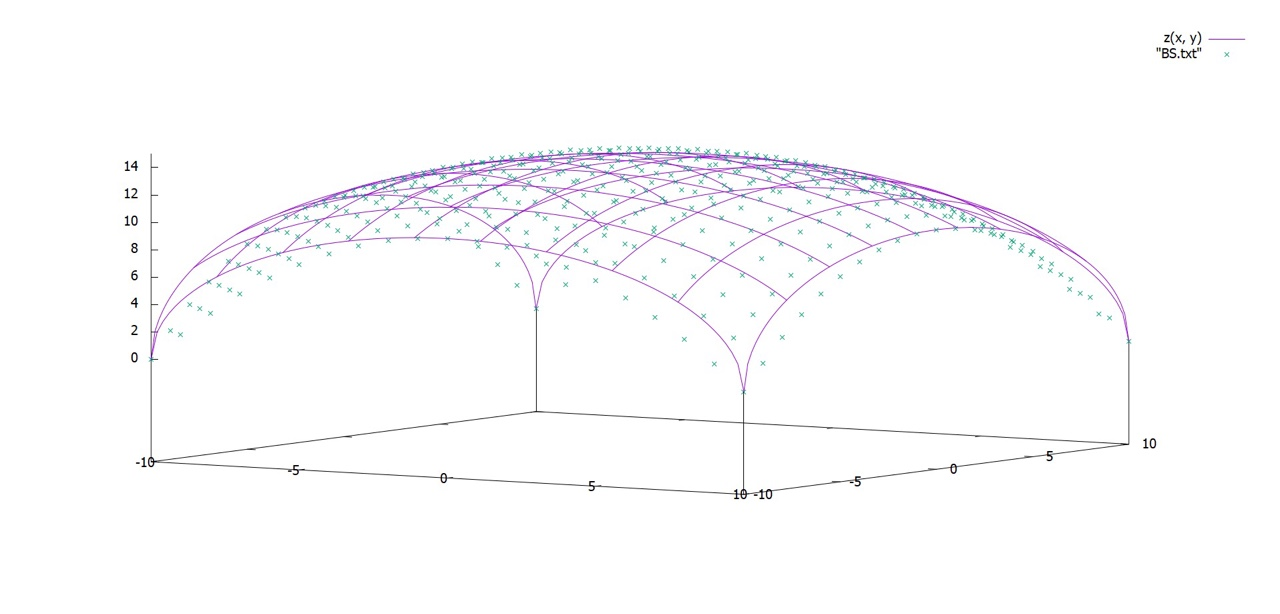
\includegraphics[width=.5\textwidth]{
		leastSquare}
	\end{center} \setstretch{1.2}
	\raggedright \small \textbf{Fig. 4. $\mathbf{b}_{11}$을 구하는 방법을 적용한 예시.} 함수 $z = \sqrt{200 - x^2 - y^2}$의 그래프에 $\mathbf{b}_{11}$을 찾는 방법을 적용한 결과이다. $\mathbf{P}_k$는 $(x, y)$가 $((2i-9)/10, \, (2j-9)/10) \ (i, j = 0, 1, \cdots, 9)$인 점이다. 베지어 곡면과 정점들 사이의 하우스도르프 거리는 약 6.32이다. 
\end{figure}

\begin{figure}[h]
	\begin{center}
		\begin{subfigure}{.2\textwidth}
			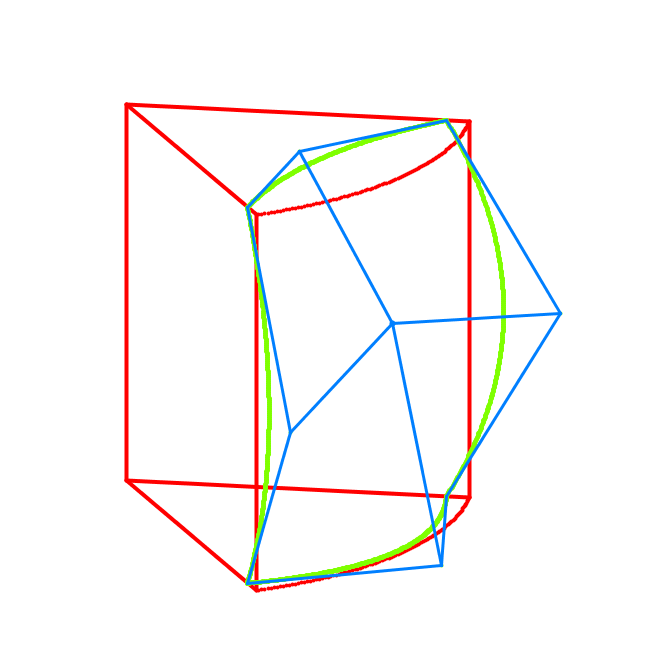
\includegraphics[width=\textwidth]{approx3}
		\end{subfigure}
		\begin{subfigure}{.2\textwidth}
			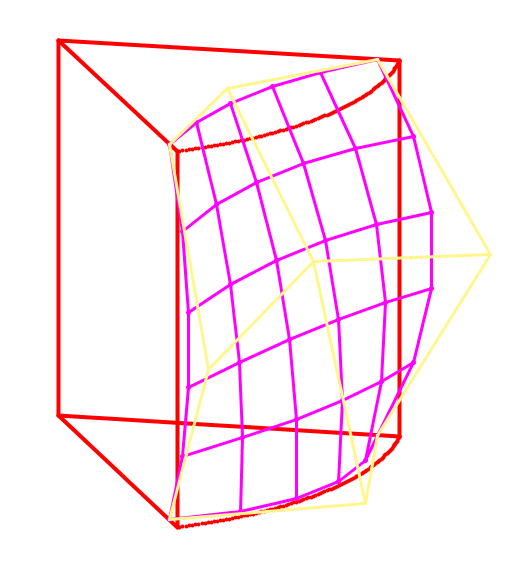
\includegraphics[width=\textwidth]{approx4}
		\end{subfigure}
	\end{center} \setstretch{1.2}
	\raggedright \small \textbf{Fig. 5. 조절점 - $\mathbf{b}_{11}$.} 최소제곱법과 가우스-뉴턴 방법을 통해 $\mathbf{b}_{11}$을 구할 수 있다. 
\end{figure}

\subsection{오차함수}
하우스도르프 거리는 거리공간 상의 두 집합이 서로 떨어진 정도를 나타내며, 오차함수로 적절하다. 그러나 \eqref{hausdorffdistance}와 같이 계산량이 많기 때문에 값을 구하는데 시간이 오래 걸린다. 본 연구에서는 이 단점을 해결하고자 하우스도르프 거리를 조금 변형해 새로운 오차함수를 정의하였다. 
\begin{defn}
	분할된 각 영역 내의 점을 $\mathbf{P}_k\ (1\leq k\leq K)$라 하고, 이에 대응되는 베지어 곡면 위의 점을 $\mathbf{x}_k$라 하자. 이때 오차함수 $\mu$는 다음과 같이 주어진다.
	\begin{equation} \label{error}
		\mu=\max_{\text{각 영역}}\max_{1\leq k\leq K} \| \mathbf{x}_k-\mathbf{P}_k \|
	\end{equation}
\end{defn}

식 \eqref{error}는 $\mathbf{P}_k$에 가장 가까운 베지어 곡면 위의 점이 $\mathbf{x}_k$라는 가정하에 \eqref{hausdorffdistance}를 다시 쓴 식이다. $\mathbf{b}_{11}$을 구하는 과정에서 $\mathbf{x}_k$와 $\mathbf{P}_k$ 사이의 차이를 작게 만들었으므로 타당한 가정이다. 

obj파일로 주어진 정점의 개수를 $N$이라 하자. 마찬가지로 베지어 곡면 위에서 $N$개의 점을 잡을 수 있다. 그러면 베지어 곡면과 obj파일로 주어진 곡면 사이의 하우스도르프 거리를 구하기 위해서는 obj파일로 주어진 정점과 베지어 곡면 위의 점의 쌍을 모두 조사해야 하므로 적어도 $O(N^2)$의 시간이 소모된다. 반면 새로운 오차함수를 구하는 시간복잡도는 $O(N)$으로, 시간이 적게 소모된다. 

\subsection{충분한 근사 가능성}
\begin{figure}[h]
	\begin{center}
		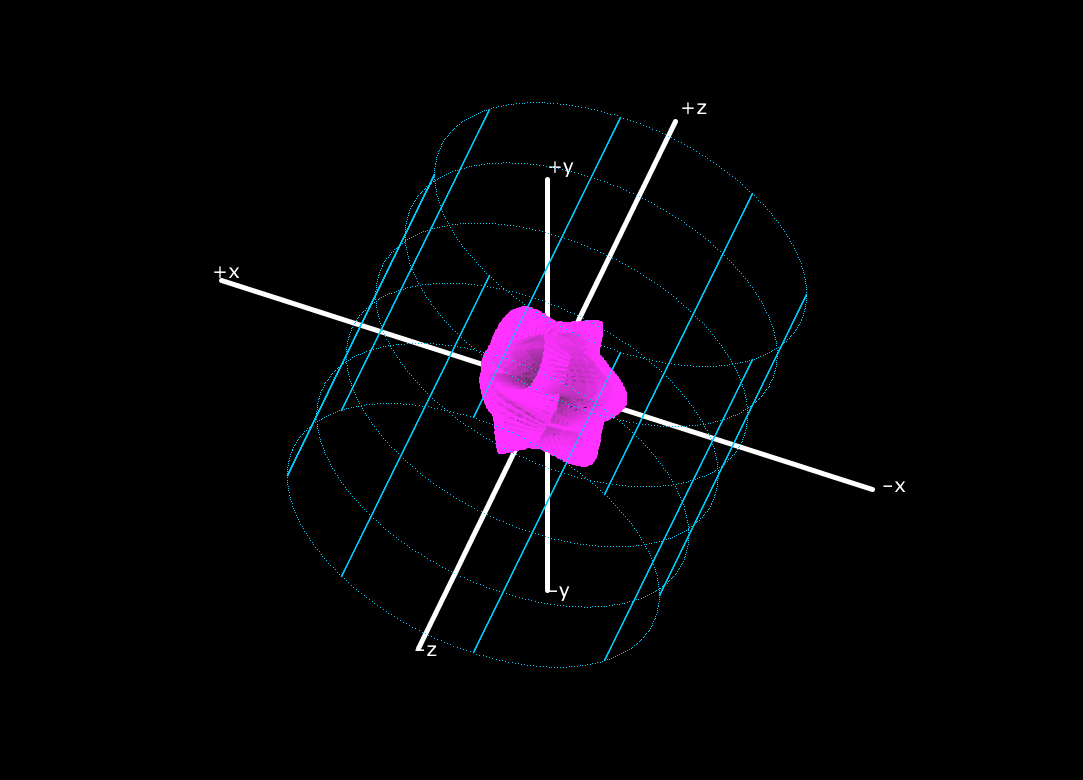
\includegraphics[width=.5\textwidth]{gg}
	\end{center} \setstretch{1.2}
	\raggedright \small \textbf{Fig. 6. 구면 근사.} 반지름이 64인 구면에 근사 방법을 적용한 모형이다. 이때 오차함수 $\mu < 10$이다. 
\end{figure}

우리는 연구 대상으로 하는 모든 곡면이 충분히 근사 가능함을 수학적으로 다음과 같이 증명하였다.
\begin{thm} \label{thm}
	위와 같은 근사 방법에 따라 3D 모델을 근사했다고 하자. 식 \eqref{error}로 주어진 오차함수 $\mu$에 대해 다음이 성립한다.
	\begin{equation*}
		\lim_{n\to\infty}\mu=0
	\end{equation*}
\end{thm} 
\begin{proof}
	$B_i^2(u) B_j^2(v)$의 합이 1이므로 다음이 성립한다.
	\begin{align*}
		\Vert \mathbf{x}_k - \mathbf{P}_k \Vert &= \left\Vert \sum_{i, j = 0}^2 B_i^2(u_k) B_j^2(v_k) (\mathbf{b}_{ij} - \mathbf{P}_k) \right\Vert \\
		&\leq \sum_{i, j = 0}^2 B_i^2(u_k) B_j^2(v_k) \Vert \mathbf{b}_{ij} - \mathbf{P}_k \Vert 
	\end{align*}
	$\Vert \mathbf{x}_k - \mathbf{P}_k \Vert$는 $\Vert \mathbf{b}_{ij} - \mathbf{P}_k \Vert$의 가중평균이므로, $\Vert \mathbf{b}_{ij} - \mathbf{P}_k \Vert \to 0$이면 $\Vert \mathbf{x}_k - \mathbf{P}_k \Vert \to 0$이다. 
	
	정리 \ref{proj}의 함수 $\mathbf{f}$를 생각하자. $\mathbf{f} \colon [0, 2\pi] \times [-h, h] \to \mathbb{R}^3$는 콤팩트 집합에서 정의된 연속함수이므로 균등연속(uniformly continuous)이다 ($\because$ Heine-Cantor theorem). 즉, 임의의 $\epsilon > 0$에 대해 다음을 만족하는 $\delta > 0$이 존재한다. 
	$$ \sqrt{(\theta - \theta^\prime)^2 + (z - z^\prime)^2} < \delta \implies \Vert \mathbf{f}(\theta, z) - \mathbf{f}(\theta^\prime, z^\prime) \Vert < \epsilon $$
	
	이제 $\mathbf{P}_k = \mathbf{f}(\theta_k, z_k)$라 하고, $(\theta_k, z_k)$를 포함하는 영역 $$ I_{ab} = \left[ \frac{2\pi a}{2^n}, \, \frac{2\pi(a+1)}{2^n}\right] \times \left[ -h + \frac{2hb}{2^n}, \, -h + \frac{2h(b+1)}{2^n} \right] $$가 $(\theta_k, z_k)$의 $\delta/2$-근방에 포함되도록 하는 최소의 자연수 $N$을 잡자. $\mathbf{b}_{00}, \mathbf{b}_{02}, \mathbf{b}_{20}, \mathbf{b}_{22} \in \mathbf{f}(I_{ab})$이므로, $n \geq N$이면 $\Vert \mathbf{b}_{00} - \mathbf{P}_k \Vert, \, \Vert \mathbf{b}_{02} - \mathbf{P}_k \Vert, \, \Vert \mathbf{b}_{20} - \mathbf{P}_k \Vert, \, \Vert \mathbf{b}_{22} - \mathbf{P}_k \Vert < \epsilon$이다. 또한 $\mathbf{f}(I_{ab})$가 $\mathbf{b}_{00}$의 $\epsilon$-근방에 포함되므로 $\Vert \mathbf{b}_{01} - \mathbf{P}_k \Vert < \Vert \mathbf{b}_{01} - \mathbf{Q} \Vert + \Vert \mathbf{Q} - \mathbf{P}_k \Vert < 2\epsilon$이 성립한다 ($\mathbf{Q}$는 3.2절 참고). 마찬가지로 $\Vert \mathbf{b}_{01} - \mathbf{P}_k \Vert, \, \Vert \mathbf{b}_{10} - \mathbf{P}_k \Vert, \, \Vert \mathbf{b}_{12} - \mathbf{P}_k \Vert, \, \Vert \mathbf{b}_{21} - \mathbf{P}_k \Vert < 2\epsilon$이다. 따라서 $(i, j) \neq (1, 1)$에 대해 $\lim_{n \to \infty} \Vert \mathbf{b}_{ij} - \mathbf{P}_k \Vert = 0$이다. 
	
	$\mathbf{b}_{11}$은 \eqref{findb11}과 같이 주어지고, 이때 $\mathbf{y}_k$는 다음과 같다.
	$$ \mathbf{y}_k = \sum_{(i, j) \neq (1, 1)} B_i^2(u_k) B_j^2(v_k) \mathbf{b}_{ij} $$ $\Vert \mathbf{b}_{11} - \mathbf{P}_k \Vert$는 아래과 같은 부등식으로 계산된다. 
	\begin{align*}
		&\Vert \mathbf{b}_{11} - \mathbf{P}_k \Vert \\
		&= \left\Vert \frac{\sum_{k=1}^K B_1^2(u_k) B_1^2(v_k) \sum_{(i, j) \neq (1, 1)} B_i^2(u_k) B_j^2(v_k) (\mathbf{P}_k - \mathbf{b}_{ij})}{\sum_{k=1}^K (B_1^2(u_k) B_1^2(v_k))^2} \right\Vert \\
		&\leq \frac{\sum_{k=1}^K B_1^2(u_k) B_1^2(v_k) \sum_{(i, j) \neq (1, 1)} B_i^2(u_k) B_j^2(v_k) \Vert \mathbf{P}_k - \mathbf{b}_{ij} \Vert}{\sum_{k=1}^K (B_1^2(u_k) B_1^2(v_k))^2} \\
		&\leq \frac{\sum_{k=1}^K B_1^2(u_k) B_1^2(v_k) (1 - B_1^2(u_k) B_1^2(v_k))}{\sum_{k=1}^K (B_1^2(u_k) B_1^2(v_k))^2} \cdot 2\epsilon \\
		&= \left[ \frac{\sum_{k=1}^K B_1^2(u_k) B_1^2(v_k)}{\sum_{k=1}^K (B_1^2(u_k) B_1^2(v_k))^2} - 1 \right] \cdot 2\epsilon \\
		&\leq \frac{K}{\sum_{k=1}^K (B_1^2(u_k) B_1^2(v_k))^2} \frac\epsilon2
	\end{align*}

	마지막 식에서 다음과 같은 절대부등식을 사용했다.
	$$ \frac{\sum x_k}{\sum x_k^2} \leq 1 + \frac{K}{4\sum x_k^2} $$
	이는 절대부등식 $x_k \leq x_k^2 + 1/4$를 변변이 더하고 $\sum x_k^2$으로 나누면 얻을 수 있다. 
	
	$u_k$와 $v_k$가 항상 $[0.01, \, 0.99]$ 범위에 있으므로 $(B_1^2(u_k) B_1^2(v_k))^2 \geq (2 \times 0.01 \times 0.99)^4 = C$이고, 이에 따라 $\Vert \mathbf{b}_{11} - \mathbf{P}_k \Vert \leq \epsilon / 2C$이다. 모든 $0 \leq i, j \leq 2$에 대해 $\lim_{n \to \infty} \Vert \mathbf{b}_{ij} - \mathbf{P}_k \Vert = 0$이므로, 이들의 가중평균인 $\mathbf{x}_k - \mathbf{P}_k$도 $n \to \infty$의 극한에서 $0$으로 수렴한다. 
	
	각 $k$에 대해서 $\lim_{n \to \infty} \Vert \mathbf{x}_k - \mathbf{P}_k \Vert = 0$이므로, 모든 $\epsilon > 0$에 대해 적당한 자연수 $N_k$가 존재해 $n \geq N_k \implies \Vert \mathbf{x}_k - \mathbf{P}_k \Vert < \epsilon$을 만족한다. 이제 자연수 $N$을 $N_k$들의 최댓값으로 정의한다. 
	$$ N = \max_{\text{각 영역}} \max_{1 \leq k \leq K} N_k $$
	그러면 모든 $n \geq N$에 대해 $\mu < \epsilon$이므로, $\lim_{n \to \infty} \mu = 0$을 얻는다. 
\end{proof}

정리 \ref{thm}는 제시한 근사 방법에 따라 obj파일로 주어진 곡면을 원하는 오차 범위 내에서 베지어 곡면으로 근사할 수 있음을 의미한다. 

\section{결론}
본 연구에서 obj파일로 정점들의 집합과 곡면을 이루는 다각형 면들이 주어졌을 때 베지어 곡면을 이용해 원 곡면을 근사한다. 이를 위해 정점들을 원통형으로 분할하며, 분할된 각 영역에 대해 베지어 곡면의 성질과 Möller–Trumbore intersection algorithm, 최소제곱법, 가우스-뉴턴 방법을 이용해 베지어 곡면을 구성하는 조절점을 얻는다. 더욱이 제시된 방법에 따라 연구 대상으로 하는 곡면들이 모두 충분히 근사될 수 있음을 보였다.

실제로 반지름의 길이가 64인 구면에 제시한 방법을 적용했을 때, 실행 시간 1분 이내에 오차함수 $\mu < 10$을 얻었고 곡면을 저장하는 메모리는 200배 이상 감소되었다. 

베지어 곡면은 삼각형 분할에 비해 더 효율적이며, 수십 배 적은 메모리를 요구한다. 그렇기에 본 연구는 VR, AR 등 곡면에 대한 그래픽 기술을 다루는 분야에서의 활용이 기대되며 특히 CAGD 분야에 있어 의미있는 결과이다. 또한 기존에 3D 모델을 저장하기 위해 자주 사용되는 obj파일을 변환시키는 연구이기에 3D 모델링이 필요한 보다 다양한 분야와 접목시킬 수 있다. 

\begin{thebibliography}{99}
	\bibitem{Farin} Farin, G. E., \& Farin, G. \emph{Curves and surfaces for CAGD: a practical guide} (Morgan Kaufmann, 2002).
	
	\bibitem{Munkres} Munkres, J. \emph{Topology} (Pearson Education, 2014)
	
	\bibitem{convex} "How can one characterize the boundary of a convex set?" ResearchGate, last modified Mar 21st, 2015, accessed Nov 28th, 2021, https://www.researchgate.net/post/How\_can\_one\_characterize \_the\_boundary\_of\_a\_convex\_set
		
	\bibitem{raytriangle} Möller, T., \& Trumbore, B. Fast, minimum storage ray-triangle intersection. \emph{Journal of graphics tools} \textbf{2(1)}, 21-28 (1997)
		
	\bibitem{last year} 윤상, 박건호. \emph{Bezier curve를 이용한 3차원 곡선의 애니메이션화} (경기과학고등학교 기초 R\&E, 2020)
		
	\bibitem{2021} Lifton, J. J., Liu, T., \& McBride, J. Non-linear least squares fitting of Bézier surfaces to unstructured point clouds. \emph{AIMS Mathematics} \textbf{6(4)}, 3142-3159 (2021)
\end{thebibliography}
	
\end{document}